% -*- coding: utf-8 -*-
% コンパイル: lualatex tr_cad.tex （2 回）
\documentclass[a4paper,10pt,twocolumn]{ltjsarticle}

\usepackage{luatexja-fontspec}
\usepackage{geometry}
\geometry{top=22mm,bottom=22mm,left=18mm,right=18mm,columnsep=7mm}
\usepackage{graphicx}
\usepackage{booktabs}
\usepackage{array}
\usepackage{amsmath,amssymb}
\usepackage{siunitx}
\usepackage{caption}
\usepackage{float}
\usepackage{enumitem}
\usepackage[hidelinks,pdfusetitle]{hyperref}
\usepackage{url}

\captionsetup{font=small,labelfont=sc,skip=4pt}
\captionsetup[table]{position=top}
\setlist{itemsep=1pt,topsep=3pt,parsep=0pt,leftmargin=1.6em}
\renewcommand{\arraystretch}{1.1}
\newcommand{\code}[1]{\texttt{\footnotesize #1}}
% ⚠ 単位は立体。数式中で \mm と書くと mm が数式イタリックになるので \mathrm で囲む。
\newcommand{\mm}{\ensuremath{\,\mathrm{mm}}}

\title{\bfseries 検査駆動によるパラメトリック CAD 設計法\\[2pt]
\normalsize\normalfont 競技ロボットの機体設計における設計妥当性の自動判定と，
その失敗様式の類型化}
\author{\normalsize 貝淵 蒼馬}
\date{\footnotesize 2026 年 8 月}

\begin{document}
\twocolumn[
\begin{@twocolumnfalse}
\maketitle
\begin{abstract}
\noindent\small
競技ロボットのような短期・少人数の機体開発では，CAD は作図の道具として用いられ，
干渉・締結・質量・加工性の妥当性は組立段階で人手により発見されることが多い。
本研究では，形状・関節・質量・製作データのすべてを単一の Python ソースから生成し，
設計の妥当性を目視ではなく 34 系統の自動検査によって判定する
検査駆動（inspection-driven）設計法を構築し，
NHK 高専ロボコン 2026 用の投擲ロボット（1{,}224 ソリッド，可動関節 12，
外形 $964\times803\times1191\mm$）の設計に適用した。

本手法の要点は三つである。第一に，部品間の固定関係を幾何ではなく宣言として保持し，
宣言と実体の突き合わせによって浮き・離れ・未宣言接触・食い込み・座面不足を
機械的に判定する。第二に，板材の外形を SIMP 法による位相最適化で決定し，
その境界条件を固定宣言の向きから自動生成する。第三に，締結要素の位置を
実体の内点判定から決定して凍結し，組立と位置決定の循環参照を断つ。

適用の結果，設計者が図面上で認識できなかった設計不良を多数検出した。
すなわち，可動部が固定部を貫通する組立不能な形状 5 件，
座面積が零である取付宣言，下穴が母材側面を $0.25\mm$ 破る締結，
線形従属な計測輪配置による横速度の不可観測性などである。
また，概算値として計上されていた締結具質量が実測の $23\,\%$ にすぎないことが判明した。
これらとは別に，自動化そのものの実装誤り（幾何の代理の実体視，
境界条件の生成規則の誤りなど）も観測されており，本稿では両者を区別して扱う。

考察では，一連の設計反復で観測された不良を六つの様式
（検査の不作動，代表姿勢基準，幾何の代理の実体視，生成物の相互依存，
数値定義の未確認，偽陽性による検査の機能停止）に類型化し，
各々に対する構成的な対策を示す。特に，検査は合格することではなく，
故意に不良を導入したときに不合格となることを確認して初めて妥当性を持つ点を強調する。

\vspace{4pt}
\noindent\textit{キーワード:} パラメトリック CAD，設計自動化，位相最適化，
干渉検査，機構設計，URDF
\vspace{10pt}
\end{abstract}
\end{@twocolumnfalse}
]

%======================================================================
\section{緒言}

競技ロボットの機体開発は，仕様の確定から製作までの期間が短く，
設計者の人数も限られる。この条件下では，CAD は「形を描く道具」として用いられ，
設計の妥当性---部品どうしが干渉しないか，締結が成立するか，
規定質量に収まるか，実際に加工できるか---は，
図面の目視と組立時の発見に委ねられることが多い。
この方式では反復のコストが物理的であり，
一つの見落としが数日単位の手戻りに直結する。

設計知識をコードとして保持する試みは知識ベース工学として体系化されているが\cite{larocca2012}，
そこでの関心は形状生成の自動化にあり，生成された形状の妥当性を
何によって判定するかは主題とされてこなかった。
市販 CAD にも干渉チェックや設計ルールチェックの機能はあるが，
それらが判定できるのは「形が重なっているか」であって，
「設計者が意図した結合が成立しているか」ではない。
接触は，締結された状態でも偶然の近接でも同じ幾何として現れるためである。
本研究が既存手法と異なるのは，意図を宣言として明示的に保持し，
宣言と実体の差を判定対象に置いた点にある。
本研究では，これに対する構成的な代替として，次の四つの原則からなる
設計法を構築した。

\begin{enumerate}[label=(\roman*)]
\item 形状はすべてコードで生成し，寸法の情報源を単一のパラメータファイルに集約する。
\item 部品間の固定関係を，幾何から推定するのではなく宣言として保持する。
\item 設計の妥当性は，宣言と実体を突き合わせる自動検査が判定する。
\item 検査で検出できなかった不良が発見された場合，
      部品ではなく検査そのものを改修する。
\end{enumerate}

本稿では，この設計法を実機規模の機体に適用した結果を報告する。
2 章で対象と制約を述べ，3 章で手法を，4--6 章で個別の要素技術
（位相最適化，締結の自動配置，妥当性検証）を述べる。
7 章に結果を示し，8 章で本手法の適用中に観測された不良を類型化して考察する。

本稿の主たる貢献は，個々の機構設計そのものではなく，
8 章に示す失敗様式の類型化にある。
すなわち，設計自動化を導入した際に生じる誤りは設計対象に固有ではなく，
少数の再現性ある様式に帰着するという知見である。
ただしこれは単一の機体・単一の設計者による観察からの帰納であり，
他の対象での再現性の確認は今後の課題である。

%======================================================================
\section{対象システムと設計制約}

\subsection{機体構成}

対象は，机上に積まれた布（雑巾）を機械的に回収し，1 枚ずつ分離して
対向ローラー方式で投擲する機体である。
走行はメカナム 4 輪，投擲は $\phi90$ の対向ローラー 2 軸，
砲塔はヨー $\pm30^\circ$・仰角 $20$--$70^\circ$，
装填はスライドレール上の櫛歯フォーク，上押さえ，ホッパー，
シンギュレータ（分離機構）で構成される。
アクチュエータは 11 軸である。
図\ref{fig:match} に，系統ごとの配置と主要寸法および規定上の基準線を示す。

\begin{figure*}[t]
\centering
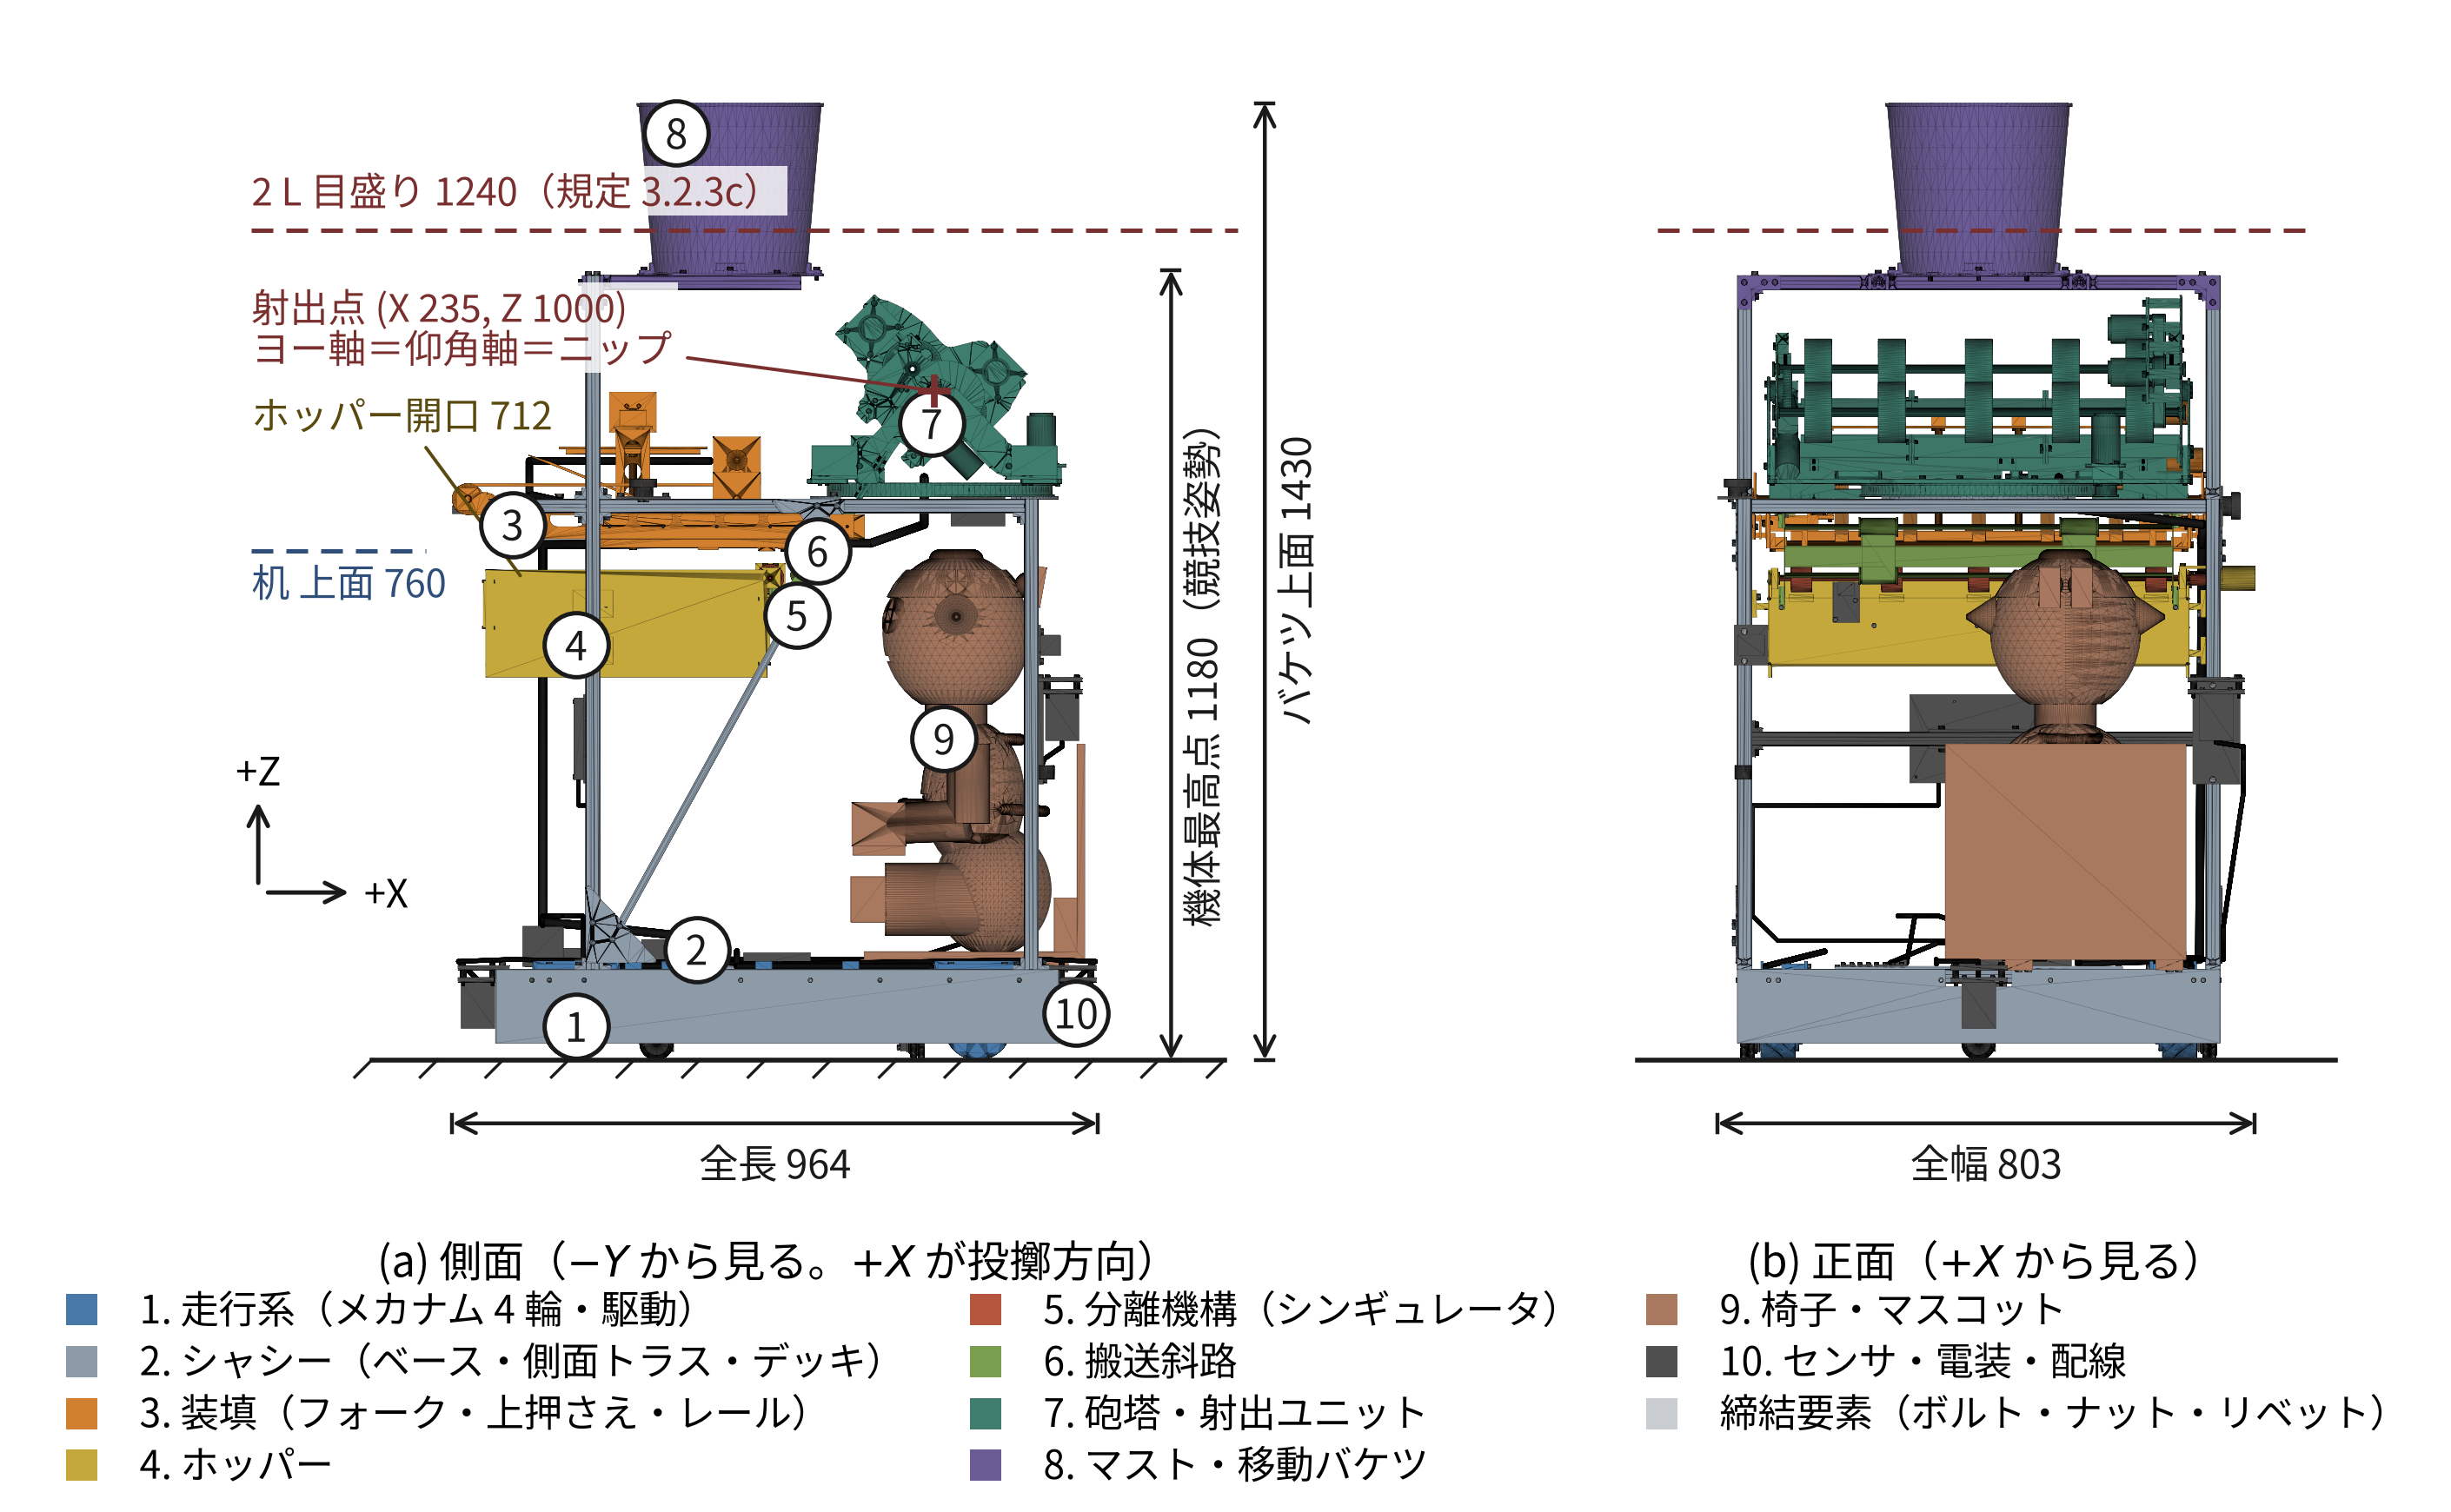
\includegraphics[width=0.97\textwidth]{figs/fig1.png}
\caption{対象機体（競技姿勢）。組立モデルの三角メッシュを正射影し，
面法線の奥行成分で陰影を与えたもので，外部レンダラを介さない。
色は系統を，白丸の番号は凡例に対応する。
締結要素は淡灰で描いている。
寸法および基準線はすべて組立モデルから実測した値であり，
図中に手入力した数値はない。
$2\,$L 目盛りの破線は，機体がこれより上に出られないという規定上の上限を示す
（2.2 節）。搭載バケツ自体はこの制限の対象外であり，破線より上に出てよい。射出点は，ヨー軸・仰角軸・ニップを一点に集めた位置であり，
砲塔をどの姿勢としても移動しない。
図は競技姿勢であり，最高点は $1180\mm$ である。
表\ref{tab:result}の $1191\mm$ は，グラバー全開などを含む
包絡で評価した規定判定値であり，姿勢が異なる。}
\label{fig:match}
\end{figure*}

\subsection{制約条件の連鎖}

本設計において最初に形状を規定したのは，性能要求ではなく
競技規定どうしの連鎖であった。関係する条項は次の三つである。
(a) スタート時の外形高さ $1200\mm$ 以内，
(b) 機体のいかなる部分も搭載バケツの $2\,$L 目盛りより上に出られない，
(c) 足回りと独立に搭載バケツを動かす機構は認められない。

(b) により，バケツ底面高さを上げない限り機体全高が $2\,$L 目盛りに拘束され，
(c) により展開機構でこれを回避できない。
したがって，バケツを展開しない固定高さとする構成が三条件を同時に満たす
唯一の解となる。設計値はバケツ上面 $1430\mm$，機体最高点 $1191\mm$，
$2\,$L 目盛り約 $1240\mm$ である。
副次的に，展開機構が不要となることで質量・剛性・故障要因の点でも有利となった。

同様に，砲塔ヨーを $\pm135^\circ$ から $\pm30^\circ$ に限定した。
粗照準を車体ヨーで生成する構成とすることで，
ホッパー・分離機構・搬送斜路を車体固定にでき，
供給経路が砲塔角に依存しなくなる。

%======================================================================
\section{設計手法}

\subsection{単一情報源のパラメトリックモデル}

形状核には OpenCASCADE\cite{occt}，記述には build123d\cite{build123d} を用いた。
全寸法をパラメータファイルの定数として保持し，
部品生成関数群がそれを参照して形状を返し，
組立モジュールが配置する構成とした。
STEP（3 姿勢），URDF，質量台帳，製作データ，各検査は
すべてこの木から導出される。
寸法変更時に編集するのはパラメータファイルのみであり，
形状記述と関節記述が同時に追従する。

\subsection{固定関係の宣言的記述}

本手法の中核は，部品配置時に固定関係を明示的に与える点にある。
配置関数は，対象部品に加えて固定先（\code{to}），
留め方（\code{how}），員数と規格（\code{note}）を受け取る。
留め方は，ボルト，溝ナット，リベット，溶接，圧入，回転対偶，
滑り対偶，貫通，載置，挟持，縫合，調整代など 20 種以上を区別する。

この宣言により，以下の判定が幾何から機械的に導出できる。
すなわち，どこにも固定されていない部品（浮き），
固定先と接触していない部品（離れ），
宣言のない接触，許容を超える干渉（食い込み），
座面積の不足，異なるリンク間を固定する不正な結合，である。

判定基準を距離から宣言へ移行させたことが初期の重要な転換点であった。
距離基準では「偶然近接している」ことと「固定されている」ことが区別できない。

留め方の区別は許容値の意味づけにも用いる。
たとえば縫合・接着による重なりの許容と，
溶接ビードによる重なりの許容は物理的に異なる現象であるため，
同一の留め方として扱うと，後に許容値を調整する根拠が失われる。
また，二枚の板が空隙をもつことが正しい調整機構については，
接触を要求しない留め方を別に定義する必要がある。
接触を要求する留め方で宣言すると必ず「離れ」と判定され，
接触するように描くと調整代が消失するためである。

\subsection{検査群}

最終的な検査群は 34 系統からなる。
主要なものを表\ref{tab:checks}に示す。
これらは一括して設計されたものではなく，
検出できなかった不良が発見されるたびに追加された。
したがって検査の一覧は，本手法の適用過程で観測された
不良様式の一覧でもある。
紙面の都合で 14 系統を挙げる。残る 20 系統（静解析，電流配分，
命中精度の誤差配分，部品表，切断リストなど）を含む全体は公開リポジトリにある。

\begin{table}[t]
\centering\footnotesize
\caption{自動検査群（主要項目）}
\label{tab:checks}
\begin{tabular}{p{0.30\linewidth}p{0.60\linewidth}}
\toprule
検査 & 判定内容\\
\midrule
規定適合 & 外形・高さ・質量・到達距離の規定値照合\\
組立整合性 & 浮き・離れ・未宣言接触・食い込み・座面・工具アクセス\\
連続掃引干渉 & 可動軸を連続に走査した際の干渉と締結の離脱\\
回転全角度 & 回転部品の全角度における干渉\\
姿勢不変性 & 姿勢によりソリッド数・部品数・宣言数が変化しないこと\\
生成物一致 & URDF・STL と組立モデルの一致\\
継手内隅 & 補強金具が入る内隅があるのに金具が無い継手\\
輪郭鮮度 & 位相最適化輪郭が現在の境界条件と整合するか\\
締結配置 & 座面積・ねじ込み側の残肉・溝中心からの偏り\\
端面タップ & ねじ山が成立する板厚か\\
荷重経路 & 肉抜きによる荷重経路の細り，継手の受け方\\
文書整合 & 組立手順書の寸法・部材長と CAD の一致\\
製作データ & 加工方法の判定可否と出力の網羅\\
動的検証 & 物理シミュレーションによる機構の成立性\\
\bottomrule
\end{tabular}
\end{table}

\subsection{凍結生成物と収束}
\label{sec:freeze}

設計の進行に伴い，組立モデルを読んでから決定される生成物が二つ生じた。
締結要素の位置と，板材の最適化輪郭である。
前者は板の外形から座面を探索し，後者は締結の座面を保存領域として解く。
すなわち両者は相互依存し，不動点をなす。

このため，一巡の再生成では収束しない。
実際，一巡のみでは「旧輪郭上に配置された締結」と
「その締結を保存して解かれた新輪郭」という不整合が残り，
組立整合性検査が固定先との離れを検出した。
二巡することで輪郭の鮮度不整合が解消した。
再生成は，締結配置，境界条件抽出，位相最適化，
メッシュ出力，URDF 出力，製作データ出力，全検査の順に実行し，
実行中はソースを変更しない規約とした。

生成物の鮮度判定にはファイル更新時刻を用いない。
ソースの些細な変更で「陳腐化」と判定されると，
真に陳腐化した際に警告が無視されるためである。
締結については配置時点の部品バウンディングボックスの指紋を，
輪郭については境界条件の指紋を用いる。

%======================================================================
\section{板材外形の位相最適化}

\subsection{肉抜き手法の変遷}

初期の軽量化は，板の外形を矩形に保ったまま円孔を配列する手法によった。
円孔は互いにリブ幅以上離し，縁から所定量離せば
残存材料が必ず連結するという構成上の利点をもつ。
しかし，連結性を孔の側で保証するため，
残存材料の幅は径とピッチの差分として与えられる。
すなわち，強度を支配する最小幅が設計値ではない。
加えて，荷重が通過しない隅部が外形の一部として残存し，
締結や接触が届く面積を実肉面積で除した値（以下，使用率）は，
板により $24$--$52\,\%$ にとどまった。

そこで，リブの網（三角格子または梯子）を先に決定し，
その間隙を除去する手法に改めた。
網は定義から連結であるため分断は構成により保証され，
リブ幅は板上のどこでも設計値に一致する。
三角格子は面内せん断に対して有利であり，
6 種 11 枚の置換で $227\,$g を削減した。

\subsection{SIMP 法の適用と境界条件の自動生成}

構造板については，孔の配置ではなく外形そのものを設計変数とすべきである。
そこで，四節点平面応力要素による有限要素解析と SIMP 法\cite{bendsoe2003}，
最適性規準法\cite{sigmund2001,andreassen2011}を実装し，密度場から切抜輪郭を生成して
CAD の面へ戻す経路を構築した。
格子依存性は密度フィルタ\cite{sigmund2007}により除去し，
フィルタ半径には最小部材半幅という製造上の意味を与えた。

境界条件は手書きせず，固定宣言の向きから生成する。
すなわち，当該板が固定されている相手を拘束，
当該板に固定されている相手を荷重，
締結の座面を密度 1 の保存領域，
板を貫通する相手を密度 0 の除去領域として与える。
図\ref{fig:topo}に出力例を示す。
13 枚の板に適用し，合計 $1.62\,$kg を削減した。

本定式化の限界を明示しておく。
荷重は自重（動的倍率 3）と横加速度（$1\,$G）のみで構成しており，
射出反力・砲塔の慣性トルク・モーター反力は含めていない。
他の検査（板の余肉，締結の成立性）と荷重の考え方を揃えるためであるが，
射出系の板については非保守側になりうる。
したがって図\ref{fig:topo}の荷重は絶対値としては小さく，
本手法が与えるのは「荷重経路に沿った形状の探索」であって，
最適化後形状に対する強度保証ではない。
強度は別途，実荷重による評価を要する。

\begin{figure}[t]
\centering
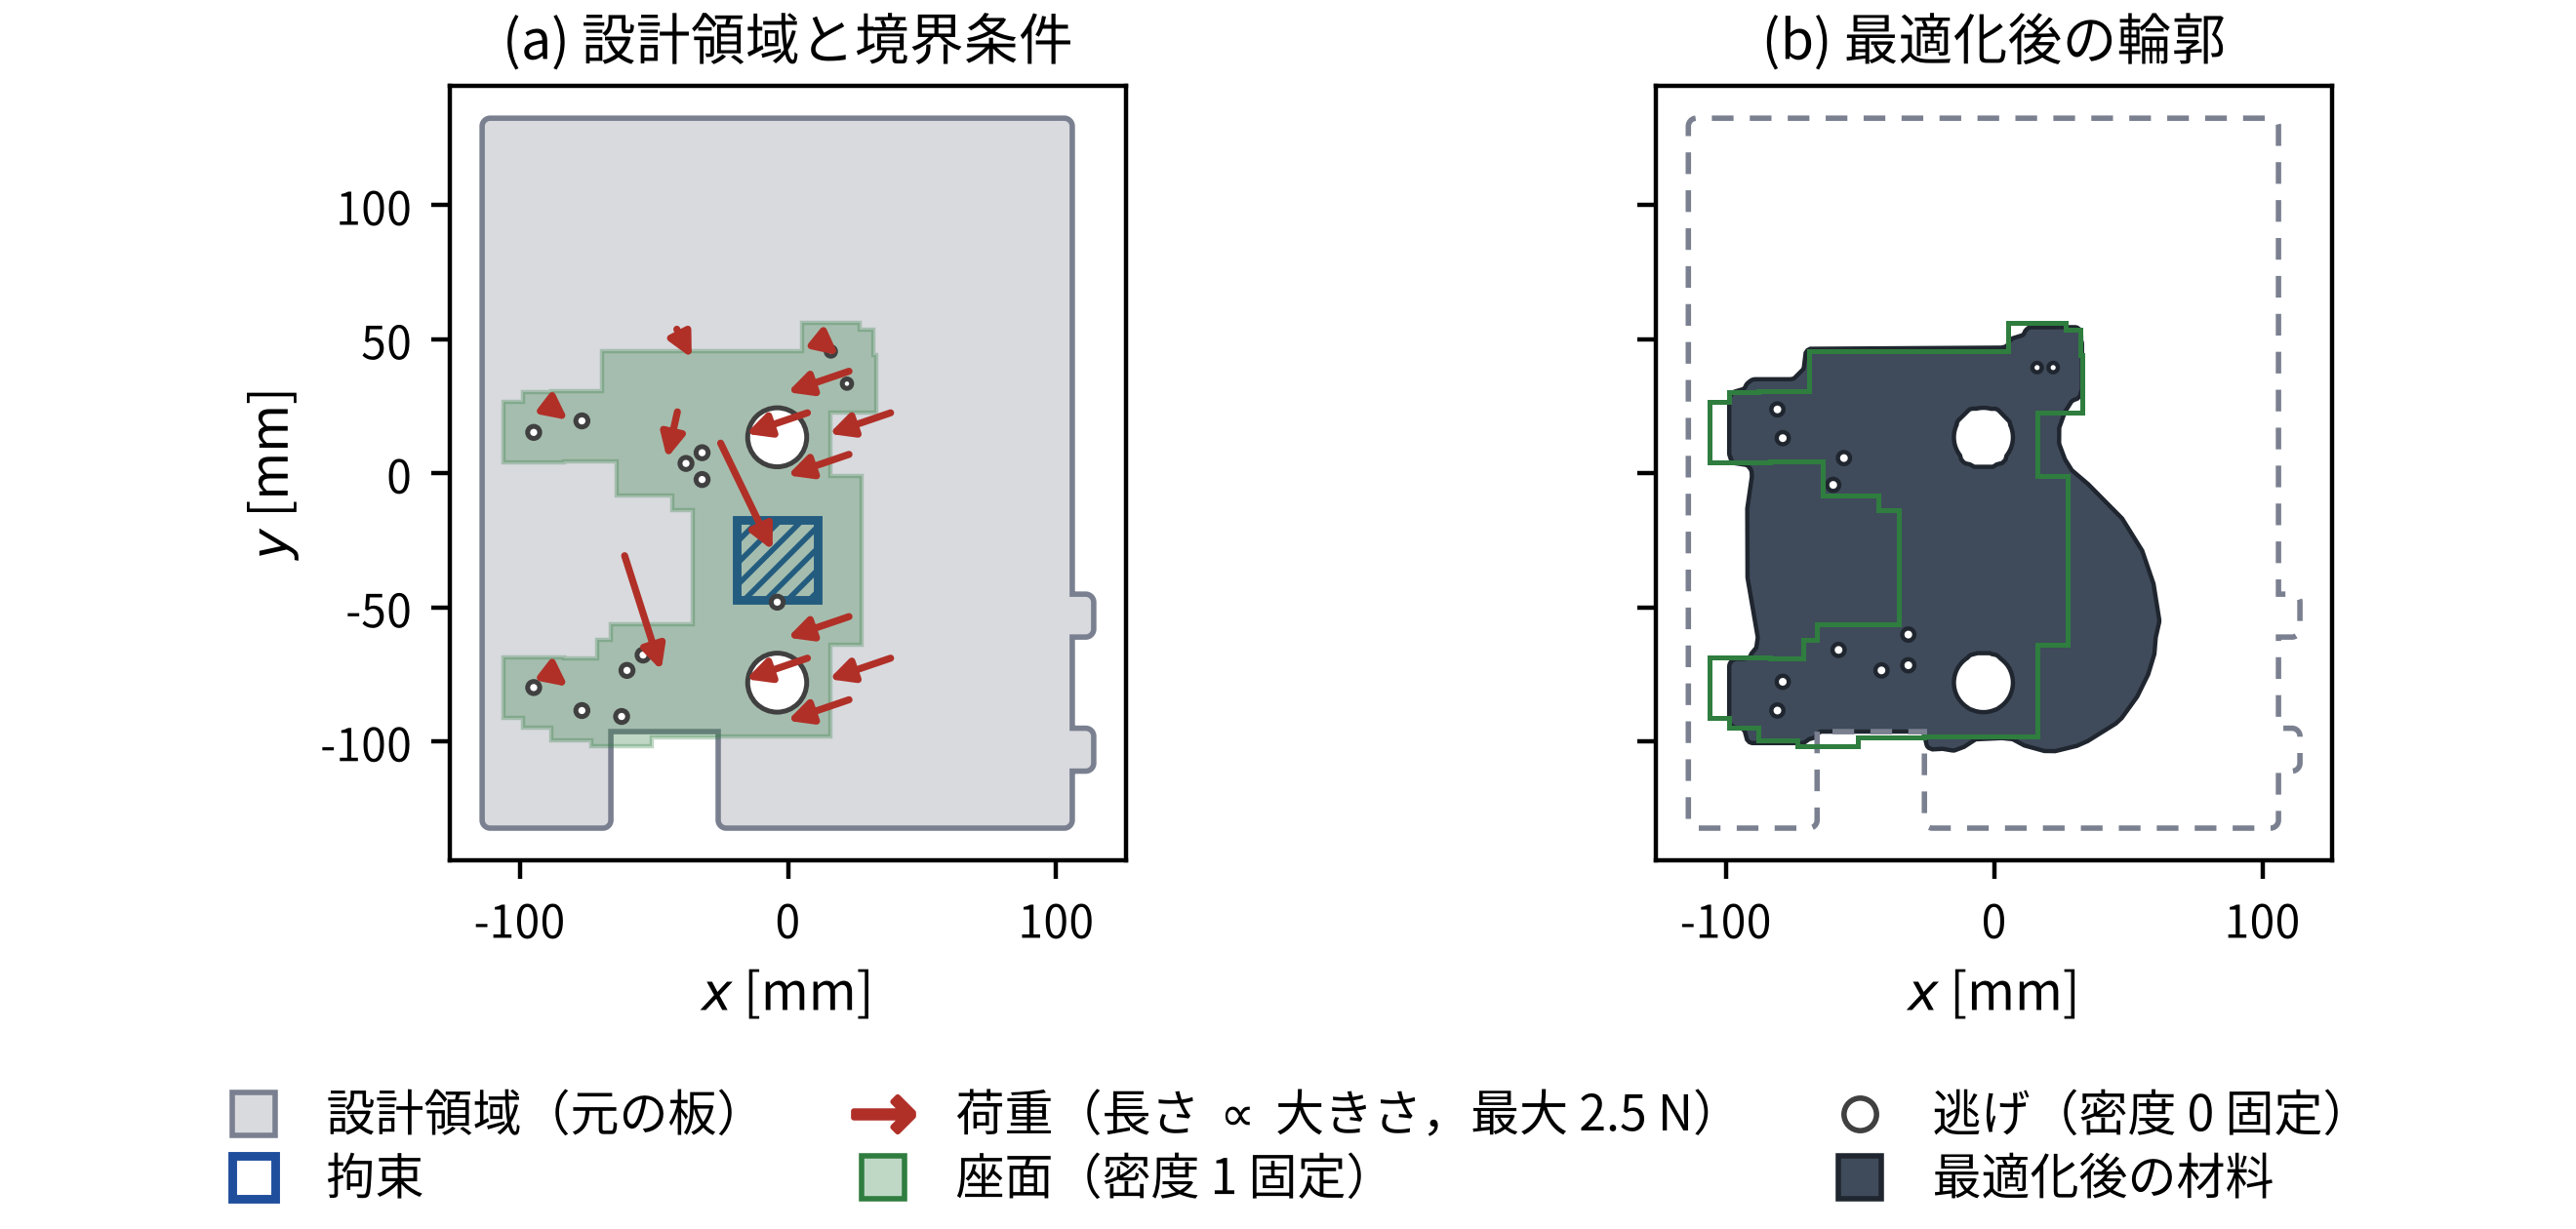
\includegraphics[width=\linewidth]{figs/fig2.png}
\caption{位相最適化の入力と出力（射出ユニット側板，$228\times265$，板厚 $3\mm$，A5052）。
(a) の境界条件は手書きではなく，固定宣言の向きから生成したものである。
矢印は個々の値ではなく荷重の作用位置と向きを示す（大きさは長さで表す）。
(b) の破線は (a) の設計領域を重ねたものである。
(b) には (a) の座面を重ねて描いた。座面の分布が最終形状の骨格に対応しており，
設計者が座面の位置を動かせば形状が変わる関係にある。
結果は面積 $19{,}291\,\si{mm^2}$，最小部材幅 $11.0\mm$，
質量 $372.5\to155.1\,$g である。
体積率 $32\,\%$ は外接矩形に対する比であり，
質量比 $41.6\,\%$（元の板に対する比）とは基準が異なる。}
\label{fig:topo}
\end{figure}

\subsection{境界条件生成における誤り}

境界条件の自動生成は，本研究で最も多くの誤りを生じた箇所である。
一般化しうる知見を以下に述べる。

第一に，固定連鎖の木における深さは，荷重の向きを与えない。
深さで拘束と荷重を分離すると，支持が零の板が生じる。

第二に，「当該板を除去したとき落下する部品を荷重とする」という定義は，
冗長構造で破綻する。左右二枚で支持する構造では，
片方を除去しても落下しないため荷重が零となる。
葉から根へ荷重を流し，分岐で等分する定義とすれば，
経路数によらず対称な結果が得られる。

第三に，板を貫通する相手を荷重から除外してはならない。
軸受は孔を通過するが，その軸受を介して被支持部材が板に懸架されている。
荷重は孔の縁で伝達されるため，孔周囲の帯として与える必要がある。
外接矩形として与えると，除去領域に囲まれた節点に荷重が載り，解が発散する。

第四に，拘束座および荷重座を保存領域に含めない場合，
最適化はそれらを除去する。荷重は節点に作用するため，
材料が存在しなくても解が成立してしまうためである。

第五に，設計領域を外接矩形とすると，元形状が矩形でない板では改悪となる。
直角三角形のガセットでは，矩形全体を使用可能とした結果，
最適化後の質量が元形状より $69\,\%$ 増加した。

\subsection{解の置換規則と最小幅の測定}

境界条件が変化すると，同一の板でも前回より重い解が得られる場合がある。
締結を実体化した結果，一枚の板の保存領域が 3 個から 27 個に増加し，
目標体積率の下限が上昇したためである。
前回輪郭でも座面は充足しているため，軽い解を採用すればよく，
より重い解では上書きしない規則を導入した。

ただし，この規則には条件が不足していた。
相手部品が移動して前回輪郭では締結が成立しない状態になった場合でも，
解が重いことを理由に据え置かれ，不成立の状態が固定される。
据え置きの条件は，書込み停止の条件より広く取る必要がある。

また，最小部材幅の測定にラスタ走査を用いると，
輪郭が細かい折線である場合に虚偽の値を返す。
画素寸法を半減させると測定値も半減し，収束しない
（測定しているのは形状ではなく格子である）。
最適化済みの輪郭では収束するため，この差が判別に利用できる。
本研究では，形態学的開処理の二分探索による幾何的測定に改めた。

\begin{figure}[t]
\centering
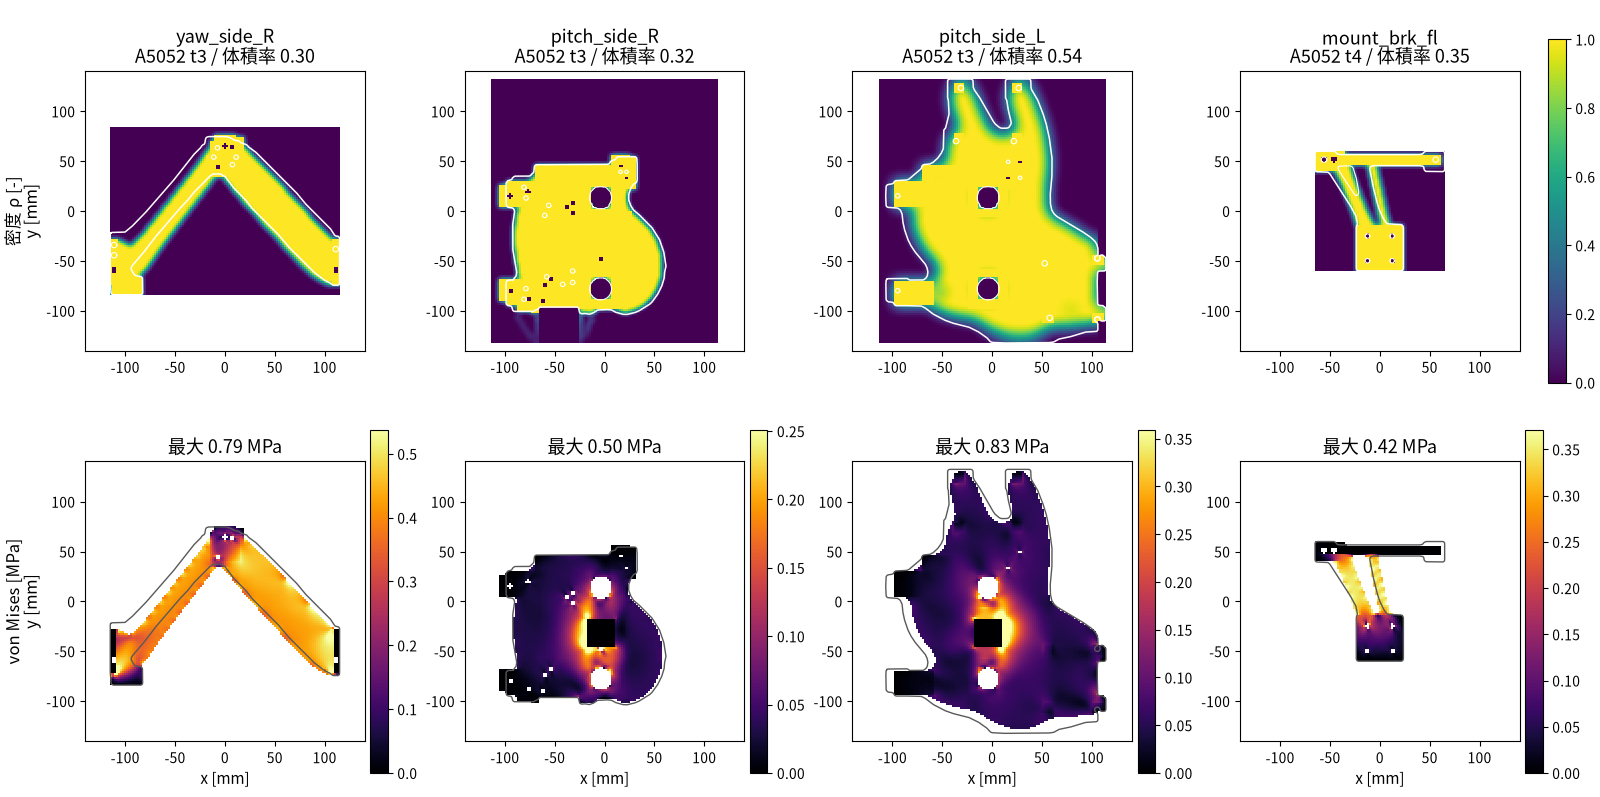
\includegraphics[width=\linewidth]{figs/heat.png}
\caption{4 枚の板の密度場（上段）と von Mises 応力（下段）。
左から，旋回アーム側板，射出ユニット側板（右・左），駆動モーターマウントである
（図中の見出しはモデル内の部品識別子）。
細線は実際に部品となった輪郭である。
最左の板は，上桁の座から斜材のボルトへ至る斜めの帯に収束し，
三角形の遠端は完全に除去されている。
応力のカラースケールは板ごとに異なる（各図の最大値で正規化）ため，
板の間で色の絶対値を比較することはできない。
また 4.2 節に述べたとおり，荷重は自重と横加速度のみであり，
応力の絶対値は実荷重に対する評価ではない。
参考として A5052 の許容応力は $90\,\si{MPa}$ 級であり，本図の値はその 1\% 以下である。}
\label{fig:heat}
\end{figure}

%======================================================================
\section{締結要素の自動配置}

\subsection{位置決定と凍結}

締結の宣言は員数と規格を含むため，質量と調達数は宣言のみから算出できる。
しかし，宣言のみでは次の三点が判定できない。
すなわち，頭部の座面が実在するか，工具が挿入できるか，
軸が第三の部品を貫通していないか，である。
ここで「組」とは締結の宣言 1 件であり，1 組は複数本のねじを含む
（たとえば「4-M5」の宣言は 4 本を意味する）。したがって組数と本数は一致しない。
本研究の初期時点で，宣言 326 組に対し実体は 148 本であり，
622 本が未実体であった。

手作業での記述は現実的でない。宣言ごとに面・座標・向き・長さを与える必要があり，
かつ相手部品が移動するたび全数を書き直すことになる。
板の外形は位相最適化により決定されるため，
手書きの座標は外形の更新と同時に無効となる。

そこで，組立モデルから位置を決定する手続きを実装した。
接触の法線を選び，接触面に格子を張り，各点の両側が
それぞれの実体内部にあるかを内点判定で確認する。
頭部の座面分だけ有効領域を収縮し，
残存点から互いに最も離れる点を選択する。
相手材の継続深さを実測して長さと留め方を決定し，
軸の通路・工具空間・近接する締結との干渉を確認する。
結果はリンク局所座標として凍結し，組立側は読み込んで配置するのみとする。
これにより組立と位置決定の循環参照を断つ。

\subsection{幾何の代理を用いたことによる誤り}

配置手続きの実装において，バウンディングボックスを実体の代理として
用いた箇所は例外なく破綻した。代表的な三例を示す。

第一に，頭部の座面高さをバウンディングボックスの外面から取得していた。
長尺の板や曲げ部品では実際の材料と無関係な値となり，
頭部が母材から $8\mm$ 浮いた状態が生じた。
上限値による飽和処理は，この破綻を緩和するのみで解決しない。
相手側の深さは実測しているのに対し，
頭部側のみが代理値のまま残されていたことが原因である。

第二に，押出材に対する締結では，溝の位置を考慮していなかった。
表面から浅い深さで材料の有無を判定すると，
溝開口部のみが候補から除外され，結果として溝を避けた位置に
締結が配置される。押出材の 84 本すべてが溝中心から $1\mm$ 以上，
最大 $6.0\mm$ 偏っていた。押出材に対しては候補を溝中心線に拘束する必要がある。
ただし，傾斜した押出材のバウンディングボックスは断面より大きいため，
この拘束は適用できない。この場合は，配置側ではなく
組立側が軸線を宣言し，検査がその軸線からの偏差を判定する構成が適切である。

第三に，候補格子の分割と収縮に関する誤りである。
接触面の重なり矩形を一定間隔で等分すると，
幅 $6\mm$ の帯では中心が格子上に存在しない。
さらに，収縮によって候補が消滅した場合に収縮前の集合へ復帰する実装では，
縁の点が候補として残存する。
その結果，下穴が母材側面を $0.25\mm$ 破る配置が生成された。
この種の不良は図面上では検出できない。孔は図面どおり加工されるためである。

対策として，分割数を奇数に強制して中心を必ず含め，
収縮半径を頭部側（頭半径）と被締結側（下穴半径と壁厚）で分離し，
候補が消滅した場合は中心線へ拘束する構成とした。
座面と残肉に関する指摘は 92 件から 16 件に減少した。
なお，この過程で判定基準を厳格化している（壁厚を固定値から呼び径比へ変更）ため，
同一基準での比較では減少幅はより大きい。

\subsection{員数の再計上}

宣言と実体を突き合わせて員数を算出した結果，
締結具は 1{,}544 個・$3{,}051\,$g であった。
質量台帳における概算値は $700\,$g であり，実測はその 4.4 倍である。
最大の項目は溝ナット M5 の 224 個・$455\,$g であった。
アルミフレーム構造では，ナットがボルトと同程度の質量を占める。

この結果，総質量は計上時点で $34.84\,$kg から $37.19\,$kg となり，規定を超過した。
増加の原因は設計変更ではなく，当初から計上していなかったことにある。
概算値に含まれている間は $160\,$g の余裕があるように見えていた。
なお，この $37.19\,$kg は締結具を数え直した時点の値である。
その後，計測輪・レベリング座・表示器・マスコットなどを
外形だけの箱から実体へ置き換えた分が加わり，
最終的な質量は表\ref{tab:result}の $39.08\,$kg となる。
以後，員数の算出は単一の関数に集約し，
質量台帳と員数表の双方がこれを参照する構成とした。

%======================================================================
\section{妥当性検証}

\subsection{機構シミュレーション}

組立モデルから生成した URDF を物理エンジン\cite{coumans2021}に読み込み，
競技環境（机，布 10 枚，教壇，標的）を配置して，
接近・挿入・引込・投入・前進・射出の一連を動的に検証した。
図\ref{fig:sim}にその一部を示す。

\begin{figure}[t]
\centering
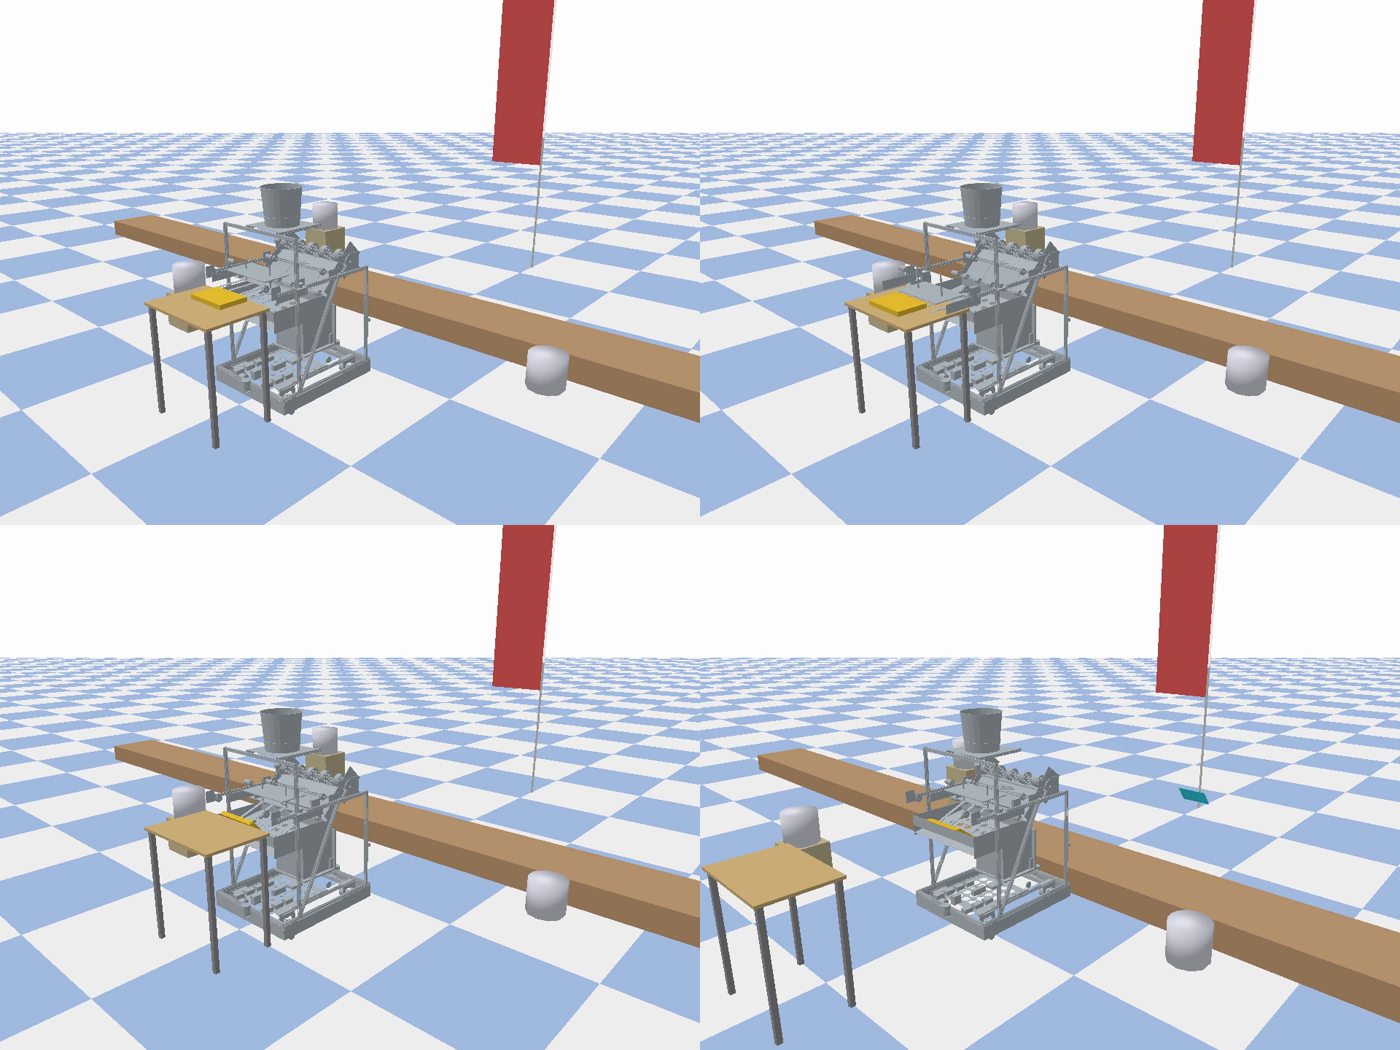
\includegraphics[width=\linewidth]{figs/frames.png}
\caption{機構シミュレーション。左上から順に，接近，挿入と引込，前進，射出。
机への接触は 0 回，机の移動量は布の摩擦による $2$--$5\mm$ にとどまる。}
\label{fig:sim}
\end{figure}

本検証は，静的な図面では検出できない 9 件の不具合を検出した。
たとえば，衝突形状を外形の単一直方体としていたため
機体が机を押し飛ばす事象，
フォーク面高さを机上面 $+5\mm$ としていたため
櫛歯が布の 1 枚目と 2 枚目の間に進入する事象，
引込後に布をホッパーへ移送する手段が存在しない事象などである。
最後の事象は，カム駆動の受動関節を追加することで
アクチュエータを増やさずに解決した。

剛体近似の限界は明示しておく必要がある。
布は剛体平板として扱われるため，たわみ・空力・はためきは表現されない。
したがって回収成功率は機構配置の妥当性を示すものであり，
実機の成功率の予測ではない。

\subsection{頑健性評価}

装填動作の頑健性をモンテカルロ法により評価した。
重要な点は，成功条件を「回収できたか」ではなく
「布の山を押さずにその下へ進入したか」まで厳格化したことである。
基準ばらつきの 2 倍までは成功率 $100\,\%$，
3 倍で $75\,\%$ に低下し，破綻点はその間にある。
これより，運用要件として山の設置精度と車体の停止精度が定量的に導かれた。

判定の厳格化は設計不良の検出にも寄与した。
緩い判定では成功と記録されていた試行において，
櫛歯が布の山を $235\mm$ 押し出していたことが判明した。
原因は，キャリッジ後端の横梁が回転軸より前方にあり，
櫛歯の上に張り出していたことである。
良好な集計値の背後で生じていた不良であり，
判定基準を厳格化しなければ検出されなかった。

\subsection{構造解析と誤差配分}

骨格を三次元梁要素で解析した結果，応力は全荷重ケースで許容値の $1/4$ 以下であり，
本機体の骨格は強度ではなく剛性で決定されていることが確認された。
ただし，照準精度に影響するのは変位そのものではなく砲塔取付面の回転であり，
さらに静的な一定成分は較正により除去できるため，
荷重ケース間の変動のみが誤差となる。
この値は $0.025^\circ$ であり，命中精度の誤差配分に対して $4\,\%$ を占めるにすぎない。
すなわち骨格剛性は命中精度の律速ではない。

一方，命中精度の誤差配分を試行回数 $2\times10^4$ のモンテカルロで求めたところ，
支配的な要因は射出初速の再現性であった。
機構の角度精度（減速機バックラッシュ）および自己位置推定は，
単独では命中率を $1\,\%$ も低下させない。
この結果は，精度への投資配分を砲塔から射出部の隙間管理へ移す根拠となった。
実際，当初想定していた偏心カムによる隙間調整は
必要分解能に対して 14 倍粗く，テーパくさび方式へ変更した。

なお，射出ローラーの軽量化は行わないという結論も本解析から得られた。
射出時の角速度低下率は，リング部の実効質量のみで決まり半径に依存しない。
低下は射出の途上で生じるため布の先端と後端で初速が変化する。
すなわちローラーの軽量化は初速再現性を直接悪化させる。

一方で，骨格剛性が支配的となる箇所も存在した。
櫛歯を布の山の下へ挿入する動作では，
机上面と歯の下面の間隙が $1.0\mm$ しかない。
片持ち量に対する先端下降量を誤差要因ごとに積み上げると，
最悪重ね合わせで $1.36\mm$ となり間隙を超過する。
ただし，下降量は片持ち量の二乗で増加するのに対し，
机の縁を通過する時点では片持ち量が全ストロークの $47\,\%$ にとどまるため，
縁における下降量は $0.53\mm$ に収まる。
奥では下降量が間隙を超えるが，そこでは歯は既に天板の上にあり，
布の下に入っている状態は変わらない。危険なのは机の縁に正面から当たる瞬間だけである。
テーパを上面のみに設けて下面を水平に保つことで，
「縁は高く越え，奥へ進むほど天板に近づく」特性が
片持ちのたわみから受動的に得られる。

%======================================================================
\section{製作データの生成}

\subsection{加工方法の判定}

設計完了時点で，加工業者に提出できる形式のファイルは存在しなかった。
そこで，組立モデルから部品を取り出し，加工方法を判定して
形式ごとに出力する経路を実装した。
判定は，体積を厚みで除した値が投影面積に一致すること
（すなわち当該軸方向に一様な板であること）を切抜の条件とし，
材質により 3D 造形を，いずれでもないものを削出・曲げとして分類する。

ここで重要なのは，判定できない部品を平板として出力してはならないことである。
外形のみもっともらしい二次元図が出力されると，
加工側はそれを信頼して加工する。
また板厚をバウンディングボックスの最小辺で決定してはならない。
曲げ部品や L 形部品では最小辺が板厚とは限らない。

曲げ部品の展開図は出力しない方針とした。
自動判定は，円筒の端面や小さな段差を「もう一枚の板」として誤認し，
部品の全長を超える辺長を返した。
より本質的には，展開長は内側曲げ半径と K 係数に依存し，
これらは加工機によって決まる。
推定値に基づく展開図の提出は，孔位置を誤ったまま確定させることに等しい。

\subsection{加工能力による形状分割とその副作用}

製作段階で，自校の加工能力が二次元切抜と端面加工に限られることが判明したため，
曲げ部品 30 点以上を平板二枚と端面ねじの組合せへ機械的に分割した。
この直後，組立整合性検査は干渉 31 件を検出し，
うち 29 件は分割によって生じた同一部品の二片間であった。

原因は明確である。曲げ部品は単一のソリッドであるため，
水平部と垂直部が隅部を共有していても矛盾しない。
分割すると，共有されていた直方体が両方の部品に帰属する。
干渉体積は必ず（幅）$\times$（板厚 a）$\times$（板厚 b）となり，
実測値がこれに一致したことで原因が特定できた。
この不良は目視では検出できない。分割後の外観は L 形のままである。

同時に，端面ねじの板厚が検査対象外であったことも判明した。
板厚 $3\mm$ の端面に M4 を指定した宣言が 8 組存在し，
ねじ山が 1.5 山しか掛からない。
孔は図面どおり加工されるため，図面上でも三次元形状上でも検出できない。

\subsection{文書の整合}

組立手順書と CAD の照合も自動化した。
検出された不整合には，部材本数の相違（22 本と 30 本），
切断リストに存在しない部材長，
$22\mm$ 異なる確認寸法，
そして同一文書内における矛盾
（ある工程が「$\phi26$ ではない」と注記する寸法を，
別の工程が「$\phi26$ を確認」と指示していた）が含まれる。
なお，設計記録文書は過去の誤った値を意図的に引用するため，
この検査の対象からは除外した。

%======================================================================
\section{結果}

最終形は 1{,}224 ソリッド，部品 1{,}185 点，可動関節 12（アクチュエータ 11 軸），
外形 $964\times803\times1191\mm$ である。
規定適合の自動判定を表\ref{tab:result}に示す。

\begin{table}[t]
\centering\footnotesize
\caption{規定適合の自動判定（最終）}
\label{tab:result}
\begin{tabular}{lrrll}
\toprule
項目 & 設計値 & 規定・目標 & 単位 & 判定\\
\midrule
スタート時外形 & $964\times803\times1191$ & $\le1000\times1000\times1200$ & mm & 適合\\
競技中最大展開 & $1189\times803\times1191$ & $\le1200\times1200\times1800$ & mm & 適合\\
搭載バケツ上面高さ & 1430 & $1200$--$2100$ & mm & 適合\\
機体最高点 & 1191 & $<1240$（$2\,$L 目盛り）& mm & 適合\\
質量 & 39.08 & $\le35.0$ & kg & 不適合\\
フォーク到達 & $-680$ & $\le-680$ & mm & 適合\\
フォーク実形状最下点 & 760.50 & $760.5$--$762$ & mm & 適合\\
ホッパー内寸 & $420\times620$ & $\ge400\times600$ & mm & 適合\\
\bottomrule
\end{tabular}
\end{table}

干渉検査は 3 姿勢 $\times$ 17 ペアで全て適合，
ここでのペアは個々のソリッドではなく，可動群と固定群の組
（砲塔$\times$側面トラス，グラバー$\times$ホッパーなど）である。
ソリッド単位の網羅は，後述の組立整合性検査と連続掃引干渉検査が担う。
組立整合性検査は浮き・分断・リンク跨ぎ・座面不足のいずれも 0 である。
製作データとして，切抜 140 点，3D 造形 31 点を出力できる状態にある。

未解決の課題は質量である。規定 $35.0\,$kg に対して $39.08\,$kg であり，
$4.08\,$kg 超過している。
列挙した削減施策の総和は $2.6\,$kg であり，全て実施しても不足する。
なお，この超過は本手法によって顕在化したものである。
締結具を計上する前は $160\,$g の余裕があるように見えており，
その余裕も，計算機を一台も計上していない見かけ上のものであった。

%======================================================================
\section{考察: 設計自動化における失敗様式}

本手法の適用過程で観測された不良は，設計対象に固有ではなく，
以下の六つの様式に帰着した。各様式について，構成的な対策を述べる。

\subsection{様式 1: 検査の不作動}

最も重大な様式である。本研究では，干渉検査が長期間にわたり
一切機能していなかった。
原因は形状ライブラリの構造にあり，子ノードは親に付与された
座標変換を自身の形状に保持しない。
本設計では可動部をグループ単位で配置していたため，
葉を直接取り出すと局所座標が返る。
干渉判定はバウンディングボックスによる粗ふるいを行うため，
一方が局所座標であれば重なりが生じず，常に「干渉なし」を返す。
すなわち可動部が関与する組合せは，すべて判定を素通りしていた。

同型の不作動は他にも複数観測された。
衝突形状にフォーク先端が含まれていなかったこと，
出力形式の変更により全リンクが「対象なし」となった検査が
無視されるようになったこと，
補強金具の宣言が員数表から意図的に除外されていたため
金具の描き忘れがどの検査にも掛からなかったこと，
掃引検査が形状のみを保存し宣言を保存していなかったことである。

対策は一つしかない。検査を追加した際に，
故意に不良を導入して当該検査が不合格を返すことを確認する。
本研究ではフォーク先端についてこれを実施し，
旧衝突形状では接触 0 回，新衝突形状では 884 回，
修正後の形状では 0 回という結果を得た。
中間の行が，検査が機能していることの証拠である。

すなわち，検査が合格することと，検査が機能していることは別である。
これはソフトウェア工学における変異テスト\cite{demillo1978,jia2011}と
同じ論法であり，本手法はそれを幾何モデルの検査へ適用したものと位置づけられる。

\subsection{様式 2: 代表姿勢を基準とすること}

逃げ量を単一の姿勢における座標から決定すると，
可動部が移動した先で必ず干渉する。
本研究では，搬送斜路，配線，締結，工具アクセスのすべてで
この様式の不良が生じた。
検査が機能を開始した時点で検出された組立不能な形状 5 件は，
すべてこの様式に属する。

対策は，掃引包絡から逆算することである。
可動範囲を走査して姿勢ごとの占有領域を求め，
固定物を配置できる限界座標を帯ごとに算出する。
本研究では，この算出により
「幅の広い砲塔を旋回させる以上，車体前半上部は旋回体に明け渡すほかない」
という幾何的結論が得られ，以後のパラメータは逆算により決定された。

なお，複数姿勢での判定には非対称性がある。
軸の通路はいかなる姿勢でも空いている必要があるが，
工具はいずれかの姿勢で挿入できればよい。
工具が必要なのは組立時のみであり，
遮蔽しているのが可動部であれば退避させればよいためである。
この区別を導入することで，配置可能な締結数が回復した。

\subsection{様式 3: 幾何の代理の実体視}

バウンディングボックスを実体として扱った箇所は，
本研究において例外なく破綻した（5.2 節）。
同様の破綻は，部品の脚部が相手の板に載っているかを
重なり矩形で判定した箇所にも生じ，
接地面の $44\,\%$ が板外へ出ている状態を適合と判定していた。
位相最適化でも，傾いた押出材のバウンディングボックスを座面として与えたため，
直角三角形のガセットの $60\,\%$ が保存領域となり，
「この板は削減できない」という誤った結論を与えていた。
座面を締結の実体から取り直すと，4 枚で $61\,$g の削減が得られた。

対策は，実体の内点判定によって測定することである。
また，バウンディングボックスが実体を代表しないことが既知の相手については，
配置側が真値を宣言し，検査がそれを参照する構成が有効である。

\subsection{様式 4: 生成物の相互依存}

相互依存する生成物は不動点をなし，一巡では収束しない
（\ref{sec:freeze}節）。
さらに，収束を保証するために導入した置換規則そのものが，
不成立な状態を固定する経路を生じさせた。

対策は，再生成順序を固定して複数巡実行すること，
据え置きの条件と書込み停止の条件を分離すること，
据え置きが発生した事実を必ず出力することである。

\subsection{様式 5: 数値定義の未確認}

外部シミュレータとの較正において，座標系の規約
（鉛直軸の取り方と原点の位置）を確認せずに解釈を先に構築したため，
必要上昇量を $0.9\,$m 過小に見積もり，較正係数が破綻していた。
規約を確認して補正係数を取り直した結果，
必要な射出速度域は当初想定の約半分となり，
ローラー回転数，蓄積エネルギー，電流要求のすべてが緩和された。

対策は，値の定義を確認する前に解釈や結論を構築しないという規律に尽きる。
本研究では，同一画面上に表示されていた別の指標との矛盾に着目することで，
誤りを検出できた例もあった。

\subsection{様式 6: 偽陽性による検査の機能停止}

ある検査は 13 枚の板について 334 件の指摘を出力していたが，
その大半は偽陽性であった。
原因は二つで，いずれも輪郭ではなく検査側の誤りである。
すなわち，設計領域の外側を評価対象に含めていたこと
（板の外に材料は置けないため，いかなる輪郭でも解消しない指摘となる），
および意図的に設けた除去領域を欠損として計上していたことである。

偽陽性は単に冗長であるだけでなく，当該検査を機能停止させる。
別の検査では，全対象が不合格となったために
「直すもの」ではなく「無視するもの」として扱われ，
その間，生成物の鮮度は誰も確認していなかった。

一方，閾値を緩和して沈黙させることも誤りである。
実測分布が連続で分離できない状況で閾値を上げ続けることは，
判定不能なものを判定しているように見せかけることに等しい。
正しい対策は測り方を変えることである。
本研究では，面積ではなく形態で評価する，
ラスタではなく幾何で測定する，
設計領域で切断してから比較する，という三つの変更により解決した。

%======================================================================
\section{結言}

本研究では，形状・関節・質量・製作データを単一のソースから生成し，
設計妥当性を 34 系統の自動検査で判定する検査駆動設計法を構築し，
実機規模の競技ロボットに適用した。

適用の結果，図面の目視では検出し得ない不良を多数検出した。
可動部が固定部を貫通する組立不能な形状，
座面積が零である取付宣言，
下穴が母材側面を破る締結配置，
線形従属な計測輪配置による特定速度成分の不可観測性，
接地面の半数近くが空中に出ている部品座などである。
また，概算値として計上されていた締結具質量が
実測の $23\,\%$ にすぎないことが判明した。

得られた最も一般的な知見は，
設計の品質が作図の丁寧さではなく，
何を機械的に問い続けたかによって決まるという点である。
同時に，検査それ自体が誤りうることを本研究は繰り返し示した。
検査は合格するだけでは信頼できず，
故意に不良を導入したときに不合格となることを確認して初めて，
設計資産として成立する。

最終形は規定適合を質量を除いてすべて満たし，
STEP 3 姿勢，URDF，二次元切抜 140 点，3D 造形 31 点を
製作データとして出力できる状態にある。
残る課題は規定質量に対する $4.08\,$kg の超過であり，
これは本手法によって概算に隠れていた質量が顕在化した結果でもある。
今後の課題は，質量制約を設計変数として最適化ループに組み込むこと，
および位相最適化を面外曲げを含む定式化へ拡張することである。

\begin{thebibliography}{99}\footnotesize
\bibitem{bendsoe2003} M. P. Bends{\o}e and O. Sigmund,
\textit{Topology Optimization: Theory, Methods and Applications},
2nd ed., Springer, 2003.
\bibitem{sigmund2001} O. Sigmund,
``A 99 line topology optimization code written in Matlab,''
\textit{Structural and Multidisciplinary Optimization},
Vol.~21, No.~2, pp.~120--127, 2001.
\bibitem{andreassen2011} E. Andreassen \textit{et al.},
``Efficient topology optimization in MATLAB using 88 lines of code,''
\textit{Structural and Multidisciplinary Optimization},
Vol.~43, No.~1, pp.~1--16, 2011.
\bibitem{sigmund2007} O. Sigmund,
``Morphology-based black and white filters for topology optimization,''
\textit{Structural and Multidisciplinary Optimization},
Vol.~33, No.~4--5, pp.~401--424, 2007.
\bibitem{demillo1978} R. A. DeMillo, R. J. Lipton and F. G. Sayward,
``Hints on test data selection: Help for the practicing programmer,''
\textit{Computer}, Vol.~11, No.~4, pp.~34--41, 1978.
\bibitem{jia2011} Y. Jia and M. Harman,
``An analysis and survey of the development of mutation testing,''
\textit{IEEE Trans. Software Engineering},
Vol.~37, No.~5, pp.~649--678, 2011.
\bibitem{larocca2012} G. La Rocca,
``Knowledge based engineering: Between AI and CAD,''
\textit{Advanced Engineering Informatics},
Vol.~26, No.~2, pp.~159--179, 2012.
\bibitem{coumans2021} E. Coumans and Y. Bai,
``PyBullet, a Python module for physics simulation for games, robotics and
machine learning,'' \url{https://pybullet.org}, 2016--2021.
\bibitem{occt} Open CASCADE Technology,
\url{https://www.opencascade.com/open-cascade-technology/}.
\bibitem{build123d} build123d,
\url{https://github.com/gumyr/build123d}.
\end{thebibliography}

\section*{公開データ}

本稿の対象機体は，CAD（STEP 3 姿勢）・URDF・製作データを公開している。
ブラウザ上で全 12 関節を動かせるビューア:\\
\url{https://3d-view.raptor-s.workers.dev/?model=/local/nhk-tr/tr.urdf}\\
STEP・URDF・製作データ:\\
\url{https://github.com/Raptor-zip/NHK-K2026/releases/tag/cad-v1.0}

\section*{謝辞・注記}

形状生成には build123d\cite{build123d} および OpenCASCADE\cite{occt} を，
動的検証には PyBullet\cite{coumans2021} を，
位相最適化の幾何処理には shapely を，
内点判定の並列化には PyTorch を用いた。
構造材の寸法は製造元の公開規格表を参照した。
本稿に記載した数値はすべて実行結果からの引用であり，
想定値については本文中にその旨を明記した。
実測により確定すべき項目は，設計記録文書において
未確定事項として管理している。

\end{document}
